%%=======================================================%%
%% to print line numbers in the margin use lineno option %%
%%=======================================================%%

%%\documentclass[lineno,sn-basic]{sn-jnl}% Basic Springer Nature Reference Style/Chemistry Reference Style

%%================================================%
%% to use numbered references, use this command %%
%%================================================%

%%\documentclass[sn-basic]{sn-jnl}% Basic Springer Nature Reference Style/Chemistry Reference Style
\documentclass[sn-mathphys]{sn-jnl}% Math and Physical Sciences Reference Style

%%\documentclass[sn-aps]{sn-jnl}% American Physical Society (APS) Reference Style
%%\documentclass[sn-vancouver]{sn-jnl}% Vancouver Reference Style
%%\documentclass[sn-apa]{sn-jnl}% APA Reference Style
%%\documentclass[sn-chicago]{sn-jnl}% Chicago Reference Style
%%\documentclass[sn-standardnature]{sn-jnl}% Standard Nature Portfolio Reference Style
%%\documentclass[default]{sn-jnl}% Default
%%\documentclass[default,iicol]{sn-jnl}% Default with double column layout

%%%% Standard Packages
\usepackage{graphicx}%
\usepackage{multirow}%
\usepackage{amsmath,amssymb,amsfonts}%
\usepackage{amsthm}%
\usepackage{mathrsfs}%
\usepackage[title]{appendix}%
\usepackage{xcolor}%
\usepackage{textcomp}%
\usepackage{manyfoot}%
\usepackage{booktabs}%
\usepackage{algorithm}%
\usepackage{algorithmicx}%
\usepackage{algpseudocode}%
\usepackage{listings}%
%%%%
\raggedbottom
%%\unnumbered% uncomment this for unnumbered level heads

\begin{document}

\title[CTRL + Style]{CTRL + Style: An Analysis of Literary Representation and Style Transfer in Transformer Models}

\author*[1]{\fnm{Your} \sur{Name}}\email{alex.tulip@studenti.unimi.it}

\affil*[1]{\orgdiv{Department of Computer Science}, \orgname{Università degli Studi di Milano}, \orgaddress{\street{Via Celoria 18}, \city{Milano}, \postcode{20133}, \country{Italy}}}

\abstract{\abstract{
The ability to understand and replicate nuanced human expression is a key challenge for large language models (LLMs). Literary style, in particular, represents a complex combination of vocabulary, syntax, tone, and narrative structure that is easy for humans to recognize but difficult for machines to quantify. This project explores the intersection of natural language processing and literary analysis by investigating how modern transformer models internally represent the distinct authorial voices of Fyodor Dostoevsky and Charles Dickens. By examining the vector space representations of their works and attempting controlled style transfer, we aim to shed light on both the capabilities and the inherent biases of these powerful models when confronted with the subtleties of literary art. Our findings indicate that a model's internal representations can effectively separate literary styles and that the success of style transfer is highly dependent on the nature of the stylistic task, with additive complexity being easier to replicate than sophisticated minimalism.
}}

\keywords{Natural Language Processing, Text Style Transfer, Literary Analysis, Transformer Models, Computational Stylometry}

\maketitle

\section{Introduction}\label{sec1}

The ability to understand and replicate nuanced human expression is a key challenge for large language models (LLMs). Literary style, in particular, represents a complex combination of vocabulary, syntax, tone, and narrative structure that is easy for humans to recognize but difficult for machines to quantify. This project explores the intersection of natural language processing and literary analysis by investigating how modern transformer models internally represent the distinct authorial voices of Fyodor Dostoevsky and Charles Dickens. By examining the vector space representations of their works and attempting controlled style transfer, we aim to shed light on both the capabilities and the inherent biases of these powerful models when confronted with the subtleties of literary art.

\section{Research Question and Methodology}\label{sec2}

\subsection{Research Question}\label{subsec2.1}
This study aims to answer the following research question: **"How do transformer models internally represent the stylistic differences between Dostoevsky's psychological realism and Charles Dickens's descriptive social commentary, and can these representations be manipulated for controlled text style transfer without altering the original text's semantic content?"**

\subsection{Measurable Objectives}\label{subsec2.2}
Our research is guided by two primary objectives:
\begin{enumerate}
    \item \textbf{Demonstrate and Quantify Stylistic Separation:} To prove that a transformer model's internal representations can effectively distinguish between the literary styles of Dostoevsky and Dickens. Our target is to achieve a classification accuracy of over 85\% based on these representations.
    \item \textbf{Achieve Controlled Style Transfer:} To successfully alter the style of a given text while preserving its core semantic content, evaluated using both automated metrics and qualitative analysis.
\end{enumerate}

\subsection{Methodology}\label{subsec2.3}
Our methodology is divided into three main phases: data curation, text embedding, and stylistic analysis.

\subsubsection{Dataset and Preprocessing}\label{subsubsec2.3.1}
A robust and clean dataset is fundamental to this analysis. We constructed a custom corpus from the full texts of major works by our chosen authors, sourced from the Project Gutenberg archive.

\begin{itemize}
    \item \textbf{Corpus Composition:}
    \begin{itemize}
        \item \textbf{Fyodor Dostoevsky:} \textit{Crime and Punishment}, \textit{The Brothers Karamazov}.
        \item \textbf{Charles Dickens:} \textit{A Tale of Two Cities}, \textit{Great Expectations}, \textit{Oliver Twist}.
    \end{itemize}
    \item \textbf{Preprocessing Pipeline:} A rigorous, multi-step cleaning process was applied to isolate the author's original writing. This involved programmatically removing Project Gutenberg headers and footers, trimming translator's notes and prefaces, and excising tables of contents. The cleaned text for each book was then segmented into paragraph-level chunks and normalized to create the final analysis-ready corpus.
\end{itemize}

\subsubsection{Text Embedding with RoBERTa}\label{subsubsec2.3.2}
To convert the textual data into a machine-understandable format, we employed a pre-trained RoBERTa-base model. Each paragraph-chunk from our corpus was fed into the model to generate a 768-dimensional vector embedding. We used the embedding of the \texttt{[CLS]} token as the representative vector for each chunk, a standard practice for capturing sentence- and paragraph-level semantics.

\subsubsection{Stylistic Analysis}\label{subsubsec2.3.3}
To test our primary hypothesis—that the embeddings of the two authors are separable—we performed a three-part analysis:
\begin{enumerate}
    \item \textbf{t-SNE Visualization:} We used t-Distributed Stochastic Neighbor Embedding (t-SNE) to visualize the embeddings in a 2D scatter plot.
    \item \textbf{Quantitative Classification:} We trained a Logistic Regression classifier on the embeddings to quantify the separability.
    \item \textbf{Conceptual Interpretation:} We used Concept Activation Vectors (CAV) to investigate if the model's separation of styles corresponded to human-understandable literary concepts.
\end{enumerate}

\section{Experimental Results}\label{sec3}

Our experiments are divided into two main parts. First, we analyze the separability of the authors' styles in a model's embedding space. Second, we test the ability of a large language model to perform controlled style transfer.

\subsection{Analysis of Stylistic Representation}\label{subsec3.1}

\subsubsection{Visualizing Stylistic Separation}\label{subsubsec3.1.1}
The t-SNE visualization of the paragraph embeddings provides strong visual evidence of stylistic separation. As shown in Figure~\ref{fig:tsne}, the embeddings form two largely distinct clusters, with minimal overlap between them. This visual separation suggests that the RoBERTa model has successfully captured distinct stylistic features for each author.

\begin{figure}[h]
    \centering
    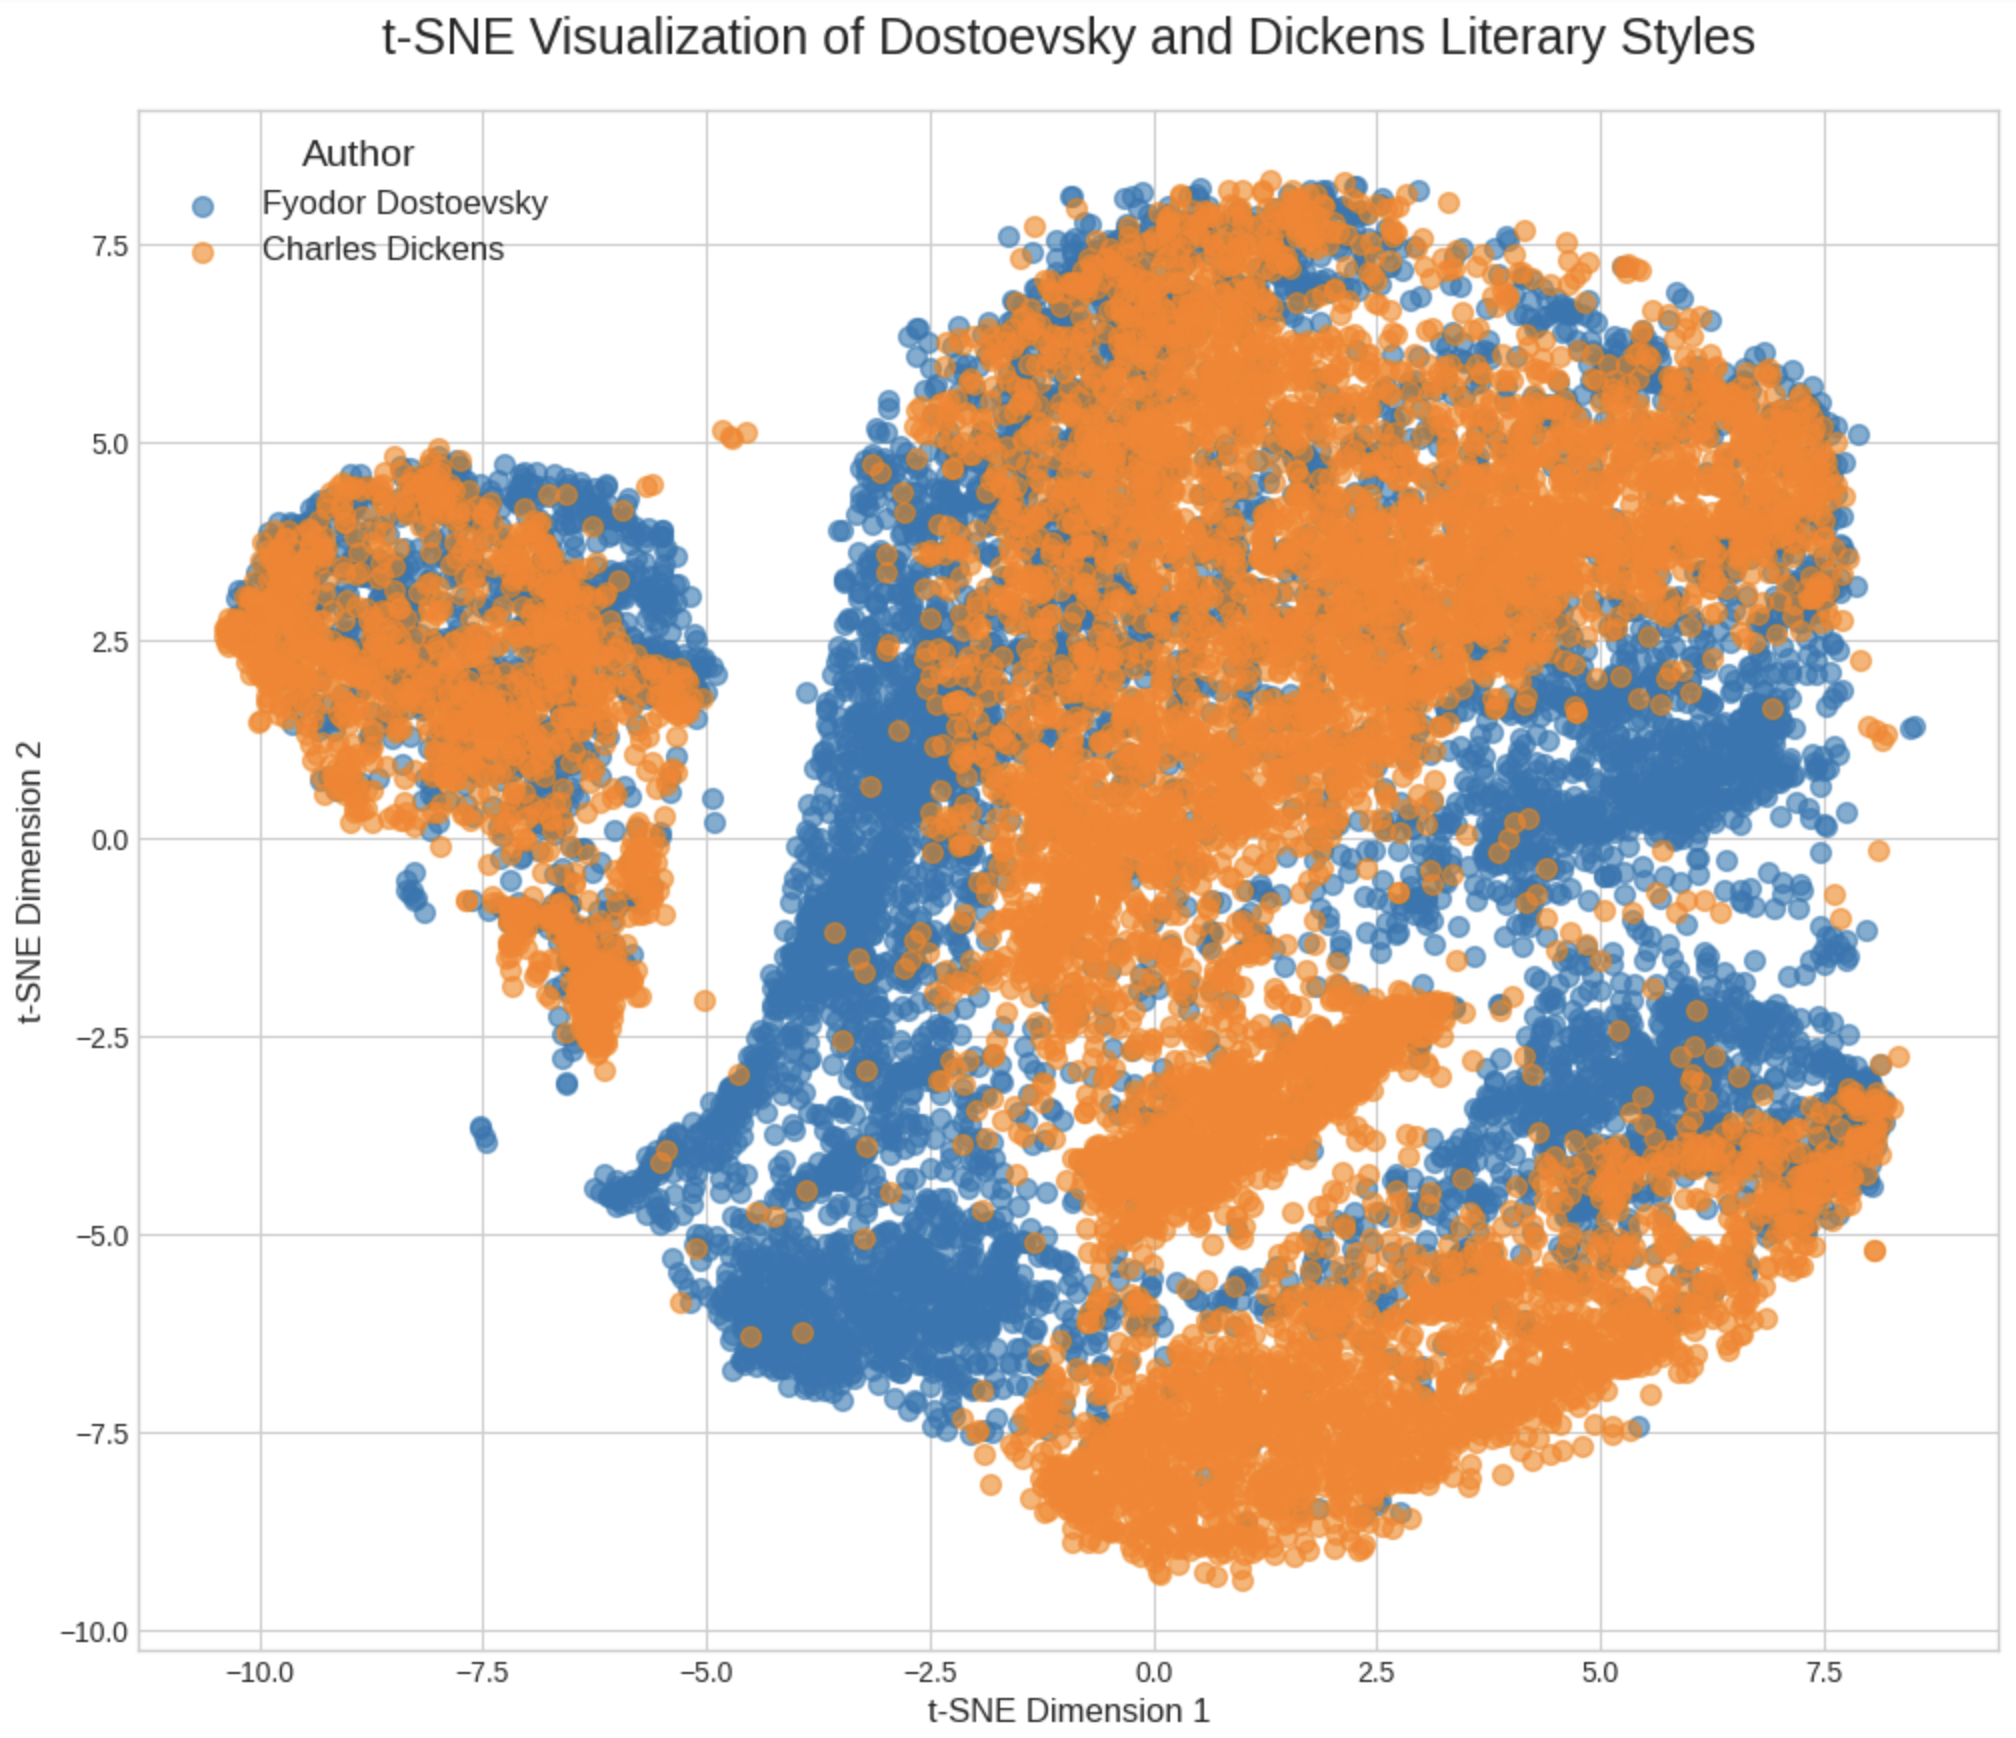
\includegraphics[width=0.8\textwidth]{t-SNE Visualisation.png} % Replace placeholder.png with your t-SNE plot image file
    \caption{t-SNE visualization of paragraph embeddings from Dostoevsky (blue) and Dickens (orange).}\label{fig:tsne}
\end{figure}

\subsubsection{Quantifying Stylistic Separation}\label{subsubsec3.1.2}
To move beyond visual intuition, we quantified the separability of the styles using a classification task. A Logistic Regression model was trained to predict the author from a paragraph's embedding alone. The model achieved an overall \textbf{accuracy of 92\%} on the held-out test set, significantly surpassing our target objective of 85\%. The detailed performance metrics in Table~\ref{tab:classification_report} and the confusion matrix in Figure~\ref{fig:confusion_matrix} provide strong quantitative evidence that the model has learned a meaningful and separable internal representation of literary style.

% You can generate this table from your classification_report output
\begin{table}[h]
\begin{center}
\begin{minipage}{\textwidth}
\caption{Classification report for predicting the author from text embeddings.}\label{tab:classification_report}
\begin{tabular*}{\textwidth}{@{\extracolsep{\fill}}lcccc@{\extracolsep{\fill}}}
\toprule
 & precision & recall & f1-score & support \\
\midrule
Fyodor Dostoevsky & 0.93 & 0.91 & 0.92 & 1604 \\
Charles Dickens   & 0.92 & 0.94 & 0.93 & 1816 \\
\midrule
accuracy & & & 0.92 & 3420 \\
macro avg & 0.92 & 0.92 & 0.92 & 3420 \\
weighted avg & 0.92 & 0.92 & 0.92 & 3420 \\
\botrule
\end{tabular*}
\end{minipage}
\end{center}
\end{table}

\begin{figure}[h]
    \centering
    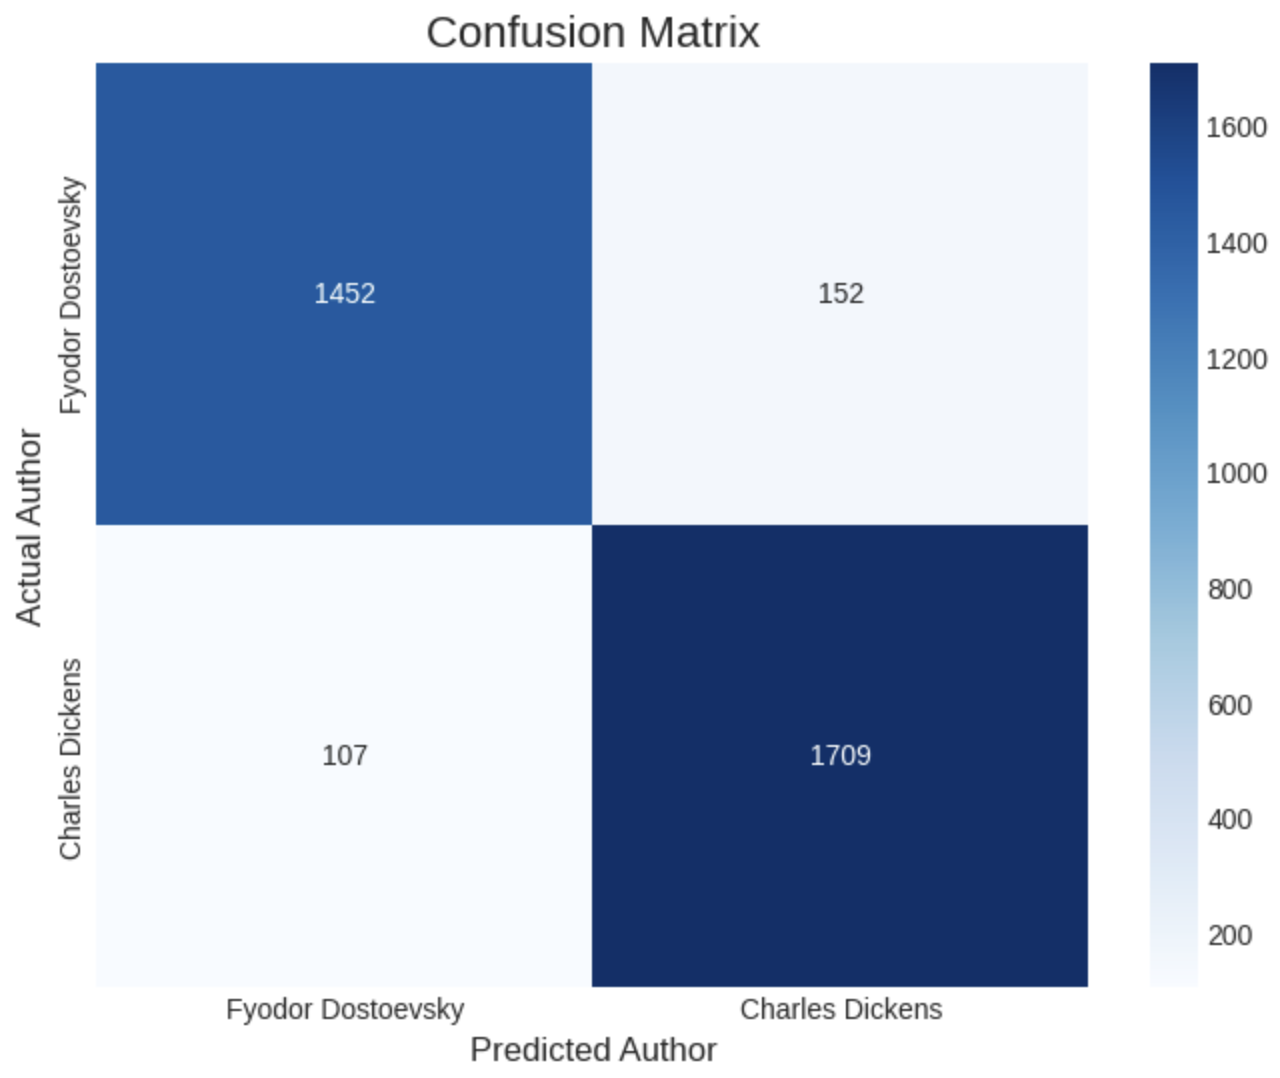
\includegraphics[width=0.6\textwidth]{Confusion Matrix.png} % Replace placeholder.png with your confusion matrix image file
    \caption{Confusion matrix for the author classification task.}\label{fig:confusion_matrix}
\end{figure}

\subsubsection{Interpreting Stylistic Dimensions with CAVs}\label{subsubsec3.1.3}
Using the CAV technique, we tested the alignment of each author's work with two concepts: "Psychological Focus" and "Social Commentary." The results (Figure~\ref{fig:cav}) reveal a clear conceptual divergence. Dostoevsky's texts showed a significantly higher sensitivity to the "Psychological Focus" concept, while Dickens's texts showed a much stronger alignment with "Social Commentary," indicating that the model's internal representations are linked to the core thematic elements of each author.

\begin{figure}[h]
    \centering
    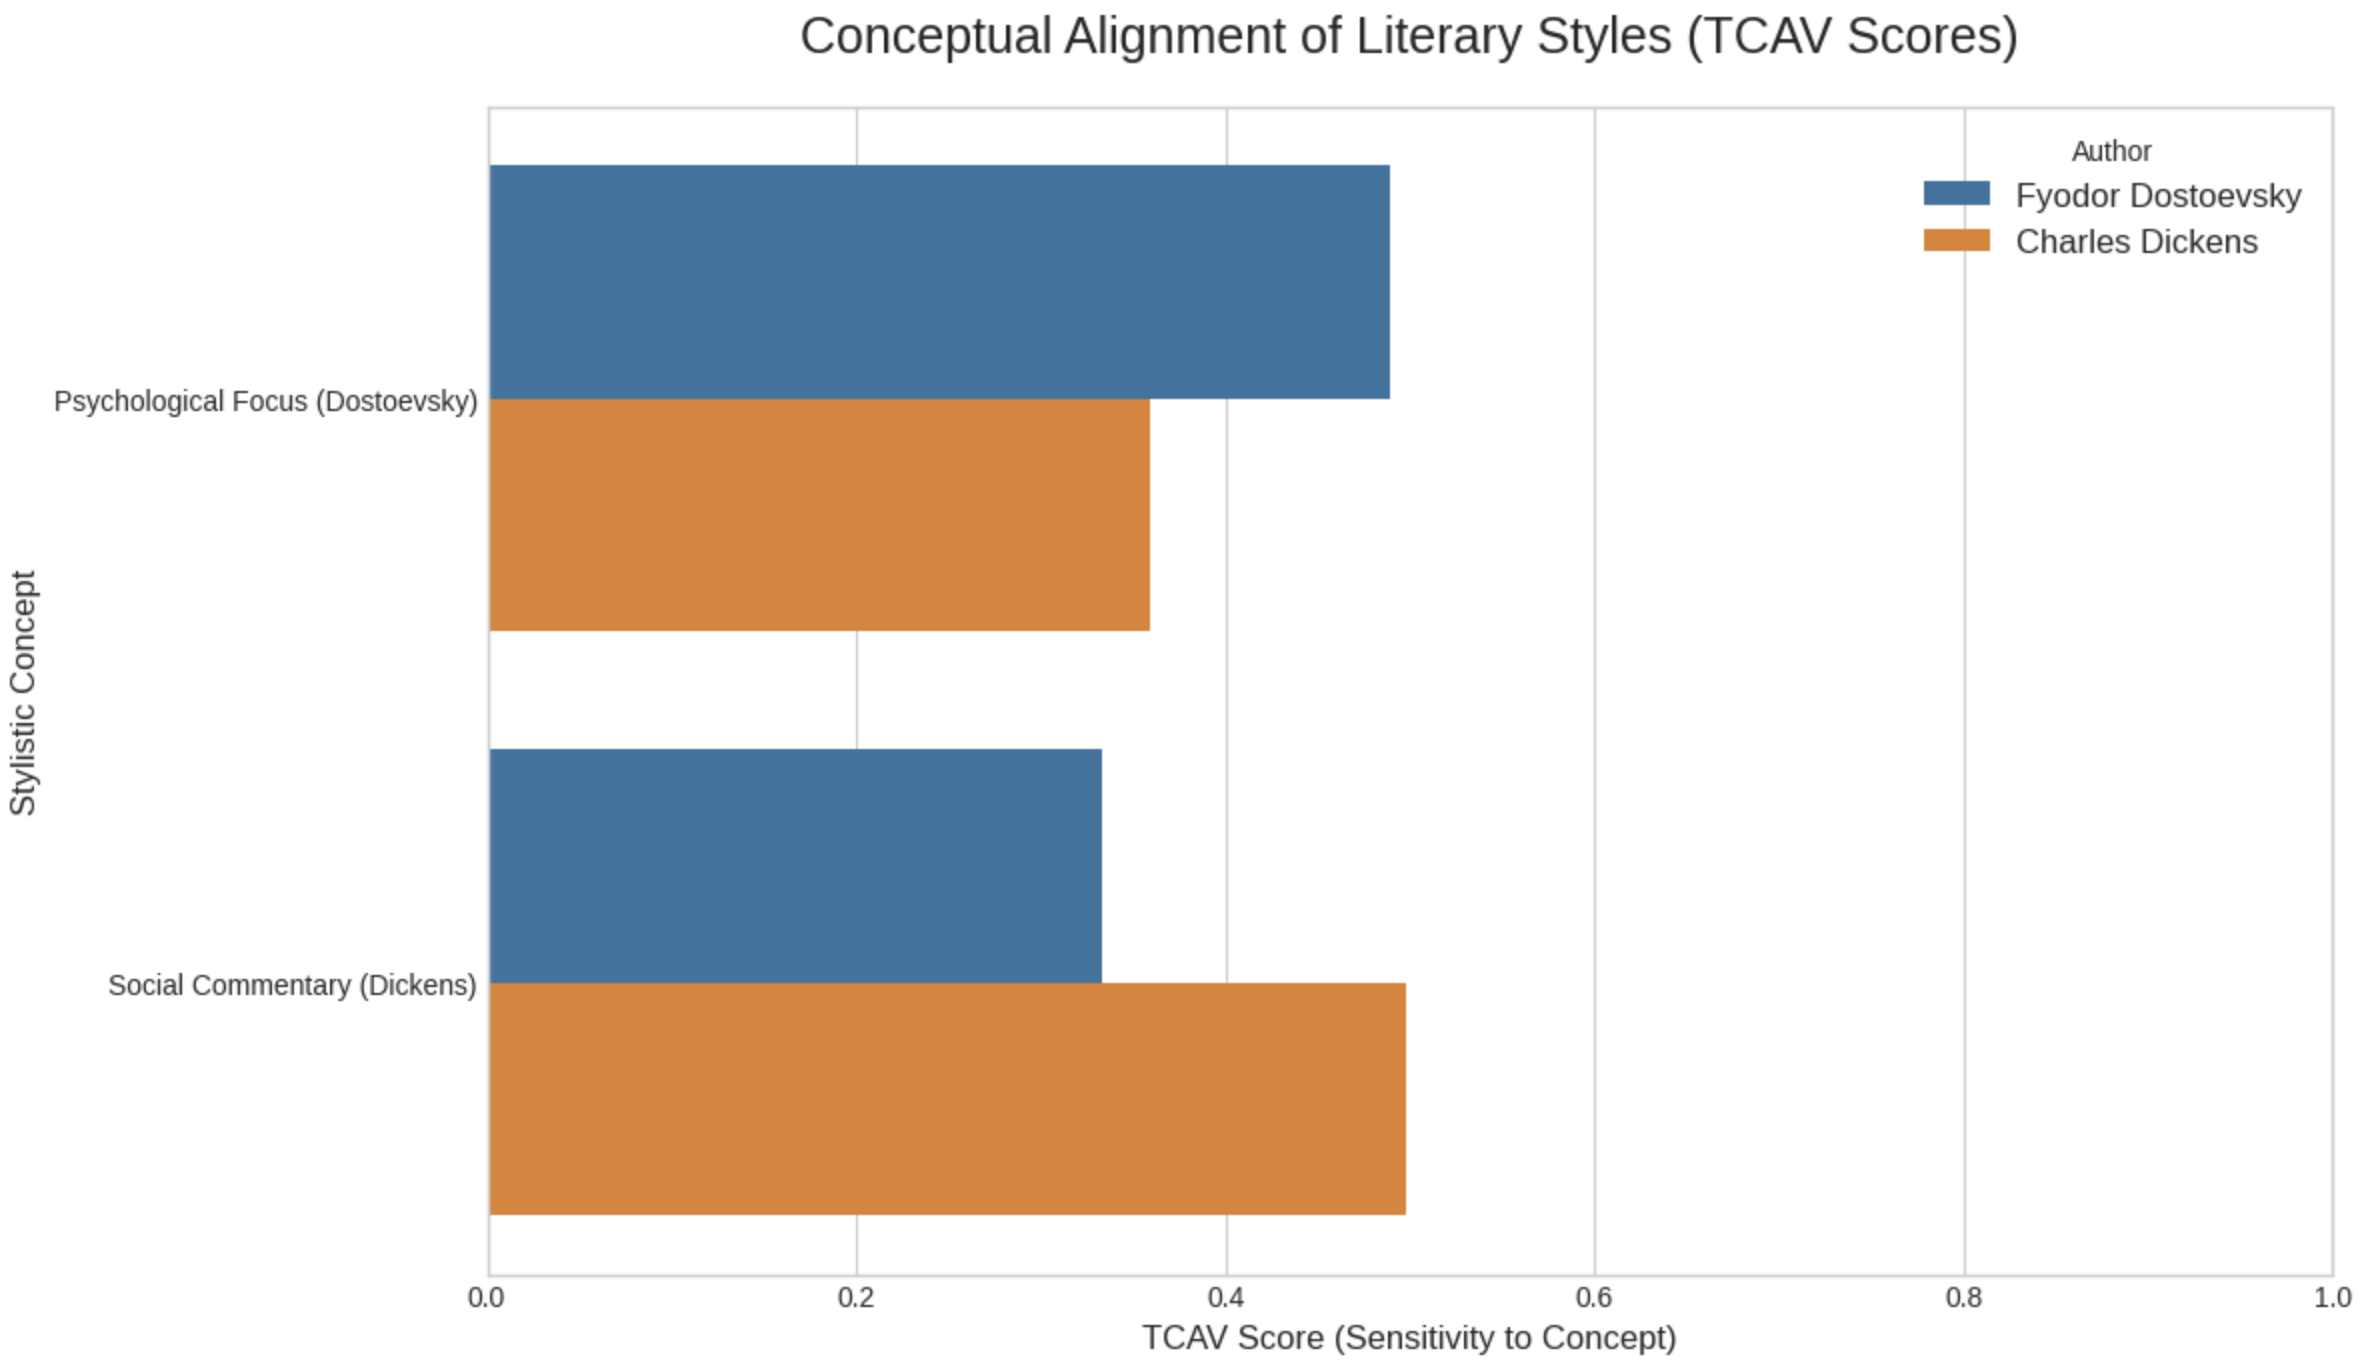
\includegraphics[width=0.8\textwidth]{CTAV Scores.png} % Replace placeholder.png with your CAV bar chart image file
    \caption{Conceptual Alignment of Literary Styles (TCAV Scores).}\label{fig:cav}
\end{figure}

\subsection{Controlled Text Style Transfer}\label{subsec3.2}

To address the second part of our research question, we explored the use of a large language model (\texttt{gemini-2.5-flash-lite-preview-06-17}) for prompt-based style transfer. We designed a detailed prompt with stylistic rules, negative constraints, and examples to guide the model. The performance was evaluated quantitatively across three metrics: Style Accuracy, Content Preservation (self-BLEU), and Fluency (Perplexity).

The results, shown in Table~\ref{tab:style_transfer_results}, reveal a significant asymmetry in the model's ability to perform style transfer between the two authors.

\begin{table}[h]
\begin{center}
\begin{minipage}{\textwidth}
\caption{Quantitative Evaluation of Style Transfer Performance (Averages).}\label{tab:style_transfer_results}
\begin{tabular*}{\textwidth}{@{\extracolsep{\fill}}llccc@{\extracolsep{\fill}}}
\toprule
From & To & Style Accuracy & self-BLEU & Perplexity \\
\midrule
Fyodor Dostoevsky & Charles Dickens & 0.84 & 0.069 & 45.72 \\
Charles Dickens   & Fyodor Dostoevsky & 0.20 & 0.066 & 70.79 \\
\botrule
\end{tabular*}
\end{minipage}
\end{center}
\end{table}

The transfer from Dostoevsky's minimalist style to Dickens's ornate style was highly successful, achieving a \textbf{Style Accuracy of 84\%}. This indicates that the model is very capable of the \textit{additive} task of enriching text with descriptive language. Conversely, the transfer from Dickens to Dostoevsky proved to be a significant challenge. The model achieved a \textbf{Style Accuracy of only 20\%}, demonstrating a clear failure to adopt the target style. This suggests that the \textit{constrictive} task of enforcing a minimalist, psychologically tense prose is much more difficult for the LLM.

\section{Concluding Remarks}\label{sec4}

This project set out to investigate whether the abstract concept of literary style could be represented and manipulated by modern transformer models. Our experiments have yielded clear and insightful results.

The first phase of our research successfully demonstrated that a pre-trained RoBERTa model can indeed learn a meaningful, internal representation of literary style, achieving a classification accuracy of 92\%. Our analysis with CAVs suggests that this separation is not arbitrary but is linked to the core thematic elements that define each author.

The second phase revealed a significant asymmetry in style transfer performance. The model was highly effective at the \textit{additive} task of transferring a minimalist style to an ornate one (84\% accuracy) but struggled significantly with the \textit{constrictive} task of adopting Dostoevsky's tense, minimalist prose (20\% accuracy).

This asymmetry is the most significant finding of our work. It suggests that while LLMs are adept at adding stylistic complexity, they have a fundamental difficulty in shedding their inherent verbosity to replicate sophisticated minimalism. This highlights a key challenge and a limitation in the current state of controlled text style transfer.

\subsection{Future Work}\label{subsec4.1}
Our findings open up several avenues for future research. One could explore more advanced style transfer techniques beyond simple prompting to see if they can better handle constrictive stylistic tasks. Another interesting direction would be to apply this methodology to a wider range of authors or even other languages to see if this additive/constrictive asymmetry is a universal phenomenon. Finally, a deeper dive into the specific linguistic features (e.g., sentence length distribution) that the model fails to replicate could provide even more granular insights into its limitations.

\begin{appendices}

\section{AI Usage Disclaimer}\label{secA1}

Parts of this project have been developed with the assistance of Google's Gemini. The AI was used to support the structuring of methodological workflows, the drafting of descriptive texts, the generation of Python code for analysis, and the refinement of experimental conclusions. All content produced with AI assistance has been carefully reviewed, edited, and validated by me. I take full responsibility for the final content and its accuracy, relevance, and academic integrity.

\end{appendices}

\end{document}
